\documentclass{beamer}
\usepackage{ulem}
\usepackage{multimedia}
\usepackage{tikz}
\usepackage{amsmath}
\usepackage{caption}
\usepackage{subcaption}
\usepackage{booktabs}
\usepackage{appendixnumberbeamer}
\usetheme{AnnArbor}
\usecolortheme{wolverine}

\title{Tube Room Update}
\author{Evan Carpenter}
\date{February 21th, 2023}
\setbeamertemplate{navigation symbols}{}

\titlegraphic{
   \begin{tikzpicture}[remember picture]
		\node[xshift=-0.3\pdfpagewidth, yshift=0.021\pdfpageheight]{
\includegraphics[width=0.17\linewidth]{atlas.png}};
		\node [xshift=0.35\pdfpagewidth, yshift=0.001\pdfpageheight]{
\includegraphics[width=0.2\linewidth]{UM.png}};
        \node [yshift=0.25\pdfpageheight, xshift=0.03\pdfpagewidth]{On behalf of the UM sMDT team};
	\end{tikzpicture}
   }
\begin{document}
\begin{frame}
	\titlepage
\end{frame}
\section{Delivery Updates}
	\begin{frame}
		\begin{block}{Delivery:}
			\begin{itemize}
				\item \small MSU delivered 192 tubes on Feb 12th. 2 Bent. 
				\item The next MSU delivery is next Friday (3/03).
			\end{itemize}
		\end{block}	
		\begin{block}{Tube Testing:}
			\begin{itemize}
				\item Mod 37 was delivered to High Bay yesterday. Mod 38 is ready and covered in Tube Room. 
				\item There are enough good tubes for Mod 39.
				\item Big update is tube swaging (next slide).
			\end{itemize}
		\end{block}
	\end{frame}


\section{Tube Room Inventory}	
		\begin{frame}{Bad Swaging Update}
			\begin{itemize}
				\item Presented video of bad swages Feb 14th. 
				\item Tested a total of 1,483 tubes. 70 tubes left to check. (276 UM tubes were sampled, but not all were tested.) 
				\item {\bf Out of 1,483 tubes checked, 445 had swage depth $>$5.40in ($30\%$ failure rate)}
				\item Evan and Claudio organized, reswaged, and tension tested 150 of the 445 bad tubes. Testing took 1 full day. 
				\item 295 left to test. Around 2-3 days. 
				\item Out of this 295, 98 are from mod 38.

			\end{itemize}
		\end{frame}
		\begin{frame}
			\begin{figure}
			\centering
			\includegraphics[width=0.75\pdfpagewidth]{Swage Depth vs. 1st Tension Date.png}
			\caption*{Swage depth of first 150 tubes Evan and Claudio re-swaged.}
			\end{figure}
			
		\end{frame}
		\begin{frame}
			\begin{figure}
				\centering
				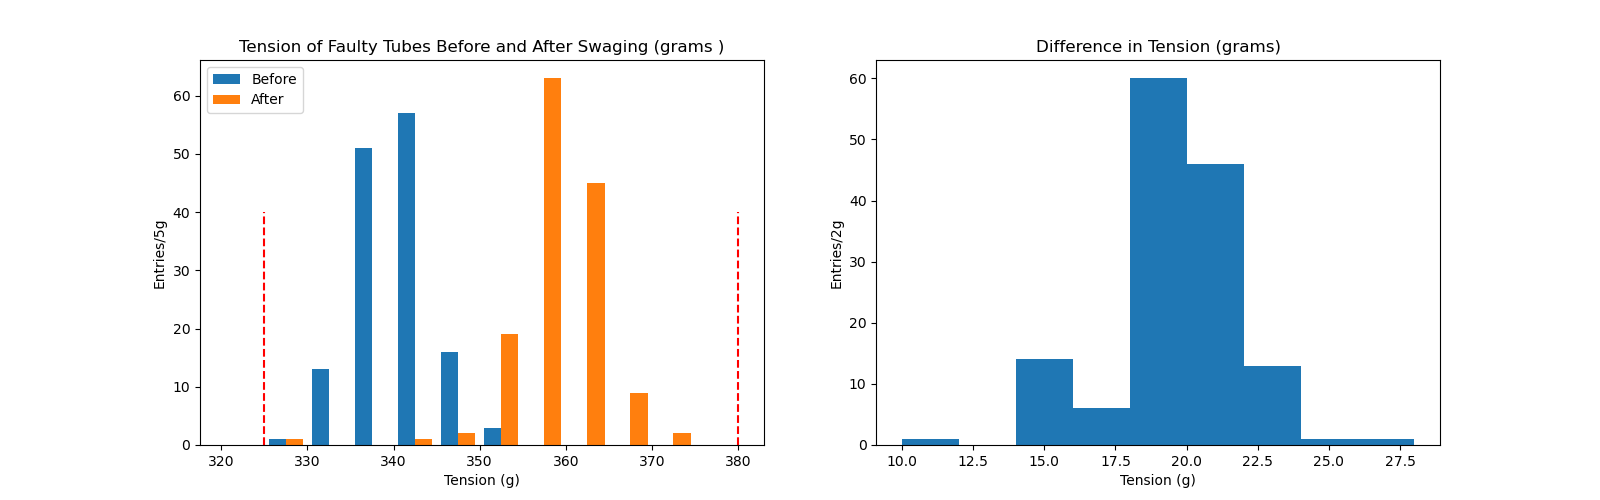
\includegraphics[width=0.9\pdfpagewidth]{TensionAfterSwaging.png}
				\caption*{Graphs showing difference in tension before and after swaging for first 150 tubes. The average rise in tension is 20g.}
			\end{figure}
		\end{frame}
		\begin{frame}
			\begin{figure}
				\centering
				\caption*{Status of Database Summary}
				\scalebox{0.6}{\begin{tabular}{r|r|r|r|r|r|r|r|r|r|r}
\toprule
           Received &  MSU &  Lost &  Bent &  LT$_\text{ok}$ &  T1$_\text{ok}$ &  T2$_\text{ok}$ &  DC$_\text{ok}$ &  Passed All &  In Chamber &  Ready \\
\midrule
(UM tubes this row) & 1359 &    19 &     9 &            1359 &            1343 &            1351 &            1353 &        1329 &        1038 &    291 \\
         2022-10-28 &  503 &    13 &    13 &             503 &             492 &             494 &             502 &         478 &         431 &     47 \\
         2022-11-04 &  100 &     1 &     1 &             100 &             100 &             100 &             100 &          99 &          81 &     18 \\
         2022-11-18 &  200 &     1 &     0 &             200 &             198 &             199 &             200 &         198 &         171 &     27 \\
         2022-11-25 &  302 &    22 &    22 &             302 &             300 &             298 &             302 &         278 &         206 &     72 \\
         2022-12-02 &  195 &    16 &    14 &             195 &             192 &             191 &             195 &         178 &         105 &     73 \\
         2022-12-09 &  100 &     3 &     2 &             100 &             100 &             100 &             100 &          97 &          66 &     31 \\
         2023-01-06 &  200 &     1 &     0 &             200 &             197 &             199 &             200 &         197 &         108 &     89 \\
         2023-01-13 &  200 &     6 &     5 &             200 &             200 &             200 &             200 &         194 &         114 &     80 \\
         2023-01-20 &  150 &     1 &     0 &             150 &             147 &             148 &             150 &         146 &           5 &    141 \\
         2023-01-27 &  100 &     0 &     0 &             100 &             100 &             100 &             100 &         100 &           0 &    100 \\
         2023-02-03 &  199 &     2 &     0 &             199 &             198 &             196 &             199 &         195 &           0 &    195 \\
         2023-02-10 &  192 &     2 &     2 &             192 &             189 &             182 &             192 &         180 &           0 &    180 \\
         2023-03-17 &  849 &     2 &     0 &             849 &             846 &             218 &             342 &         215 &           0 &    215 \\
              Total & 4649 &    89 &    68 &            4649 &            4602 &            3976 &            4135 &        3884 &        2325 &   1559 \\
\bottomrule
\end{tabular}
}
			\end{figure}
			\begin{itemize}
				\item Mod 37 and 38 counted as Ready.
				\item After Mod 37,38: $>$606 ready.
			\end{itemize}
				

		\end{frame}
		
		\begin{frame}
			%\frametitle{Tube Room Inventory - UM Tubes}
			\begin{figure}
				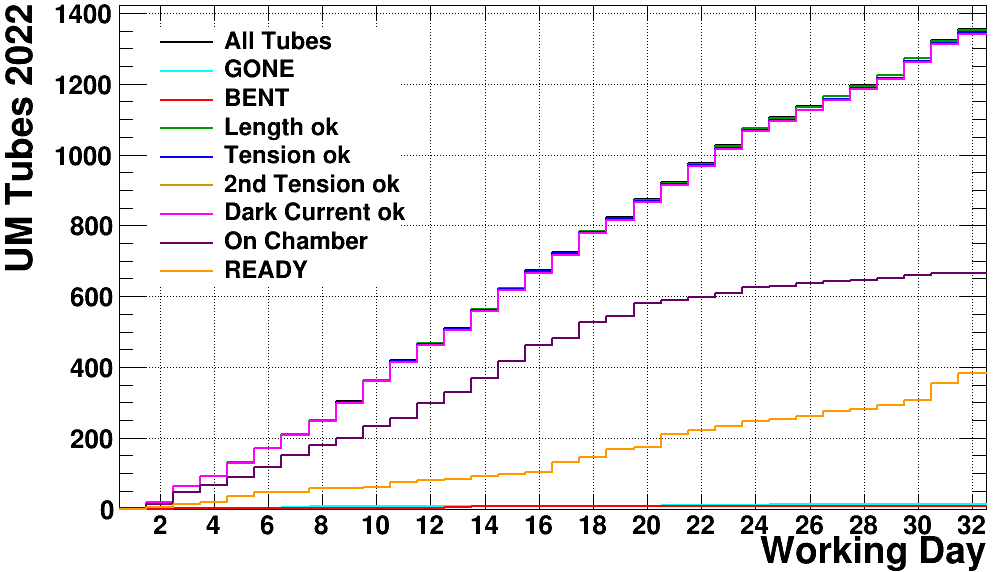
\includegraphics[width=\linewidth]{/Users/evan/Library/CloudStorage/GoogleDrive-ecarp@umich.edu/Shared drives/sMDT Tube Testing Reports/TubeMadeAtUM/UMdaily2022.png}
			\end{figure}
		\end{frame}
\appendix
\begin{frame}{All Tubes}
	\begin{figure}
		\centering
		\scalebox{0.6}{\begin{tabular}{r|r|r|r|r|r|r|r|r|r|r}
\toprule
           Received &  MSU &  Lost &  Bent &  LT$_\text{ok}$ &  T1$_\text{ok}$ &  T2$_\text{ok}$ &  DC$_\text{ok}$ &  Passed All &  In Chamber &  Ready \\
\midrule
(UM tubes this row) & 1359 &    19 &     9 &            1359 &            1343 &            1351 &            1353 &        1329 &        1038 &    291 \\
         2022-10-28 &  503 &    13 &    13 &             503 &             492 &             494 &             502 &         478 &         431 &     47 \\
         2022-11-04 &  100 &     1 &     1 &             100 &             100 &             100 &             100 &          99 &          81 &     18 \\
         2022-11-18 &  200 &     1 &     0 &             200 &             198 &             199 &             200 &         198 &         171 &     27 \\
         2022-11-25 &  302 &    22 &    22 &             302 &             300 &             298 &             302 &         278 &         206 &     72 \\
         2022-12-02 &  195 &    16 &    14 &             195 &             192 &             191 &             195 &         178 &         105 &     73 \\
         2022-12-09 &  100 &     3 &     2 &             100 &             100 &             100 &             100 &          97 &          66 &     31 \\
         2023-01-06 &  200 &     1 &     0 &             200 &             197 &             199 &             200 &         197 &         108 &     89 \\
         2023-01-13 &  200 &     6 &     5 &             200 &             200 &             200 &             200 &         194 &         114 &     80 \\
         2023-01-20 &  150 &     1 &     0 &             150 &             147 &             148 &             150 &         146 &           5 &    141 \\
         2023-01-27 &  100 &     0 &     0 &             100 &             100 &             100 &             100 &         100 &           0 &    100 \\
         2023-02-03 &  199 &     2 &     0 &             199 &             198 &             196 &             199 &         195 &           0 &    195 \\
         2023-02-10 &  192 &     2 &     2 &             192 &             189 &             182 &             192 &         180 &           0 &    180 \\
         2023-03-17 &  849 &     2 &     0 &             849 &             846 &             218 &             342 &         215 &           0 &    215 \\
              Total & 4649 &    89 &    68 &            4649 &            4602 &            3976 &            4135 &        3884 &        2325 &   1559 \\
\bottomrule
\end{tabular}
}
		\\
		\vspace{0.5cm}
		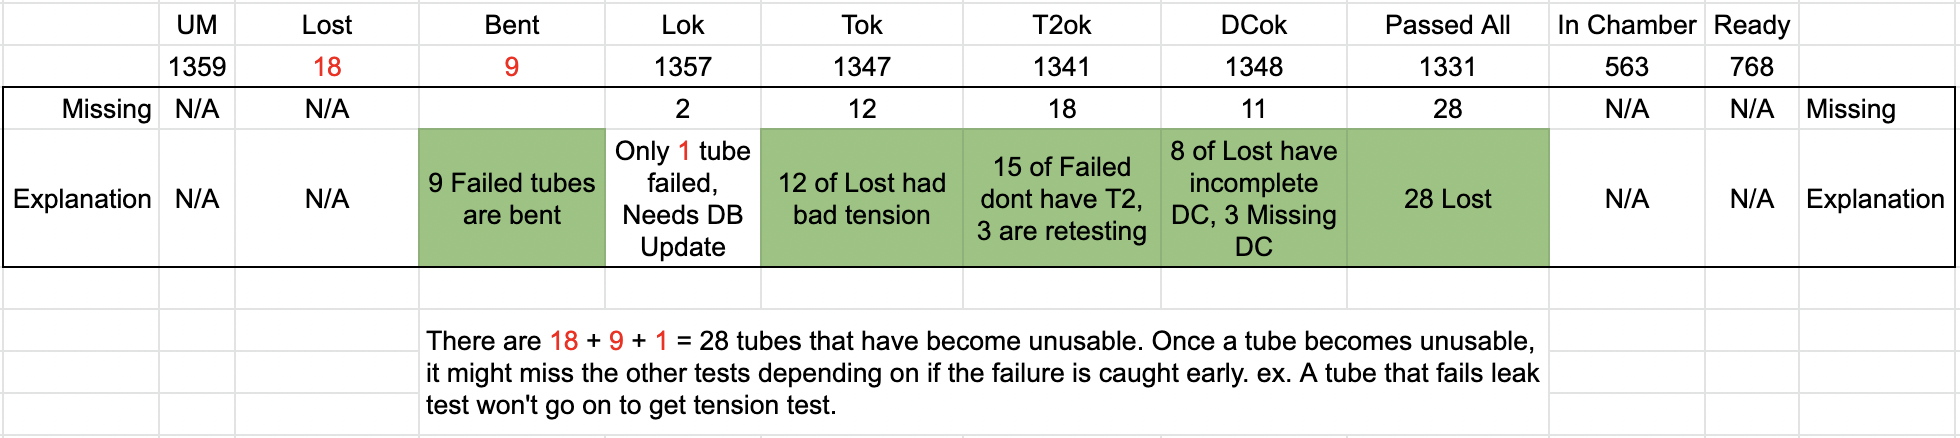
\includegraphics[width=0.8\pdfpagewidth]{UMMissingTubeExplanation.png}
	\end{figure}
	
\end{frame}
	\begin{frame}
		\centering\bf Tests of automating summary-making process.
	\end{frame}
	\begin{frame}{Tube Room Inventory - All Tubes}
		\begin{figure}
			\centering
			\scalebox{0.6}{\begin{tabular}{r|r|r|r|r|r|r|r|r|r|r}
\toprule
           Received &  MSU &  Lost &  Bent &  LT$_\text{ok}$ &  T1$_\text{ok}$ &  T2$_\text{ok}$ &  DC$_\text{ok}$ &  Passed All &  In Chamber &  Ready \\
\midrule
(UM tubes this row) & 1359 &    19 &     9 &            1359 &            1343 &            1351 &            1353 &        1329 &        1038 &    291 \\
         2022-10-28 &  503 &    13 &    13 &             503 &             492 &             494 &             502 &         478 &         431 &     47 \\
         2022-11-04 &  100 &     1 &     1 &             100 &             100 &             100 &             100 &          99 &          81 &     18 \\
         2022-11-18 &  200 &     1 &     0 &             200 &             198 &             199 &             200 &         198 &         171 &     27 \\
         2022-11-25 &  302 &    22 &    22 &             302 &             300 &             298 &             302 &         278 &         206 &     72 \\
         2022-12-02 &  195 &    16 &    14 &             195 &             192 &             191 &             195 &         178 &         105 &     73 \\
         2022-12-09 &  100 &     3 &     2 &             100 &             100 &             100 &             100 &          97 &          66 &     31 \\
         2023-01-06 &  200 &     1 &     0 &             200 &             197 &             199 &             200 &         197 &         108 &     89 \\
         2023-01-13 &  200 &     6 &     5 &             200 &             200 &             200 &             200 &         194 &         114 &     80 \\
         2023-01-20 &  150 &     1 &     0 &             150 &             147 &             148 &             150 &         146 &           5 &    141 \\
         2023-01-27 &  100 &     0 &     0 &             100 &             100 &             100 &             100 &         100 &           0 &    100 \\
         2023-02-03 &  199 &     2 &     0 &             199 &             198 &             196 &             199 &         195 &           0 &    195 \\
         2023-02-10 &  192 &     2 &     2 &             192 &             189 &             182 &             192 &         180 &           0 &    180 \\
         2023-03-17 &  849 &     2 &     0 &             849 &             846 &             218 &             342 &         215 &           0 &    215 \\
              Total & 4649 &    89 &    68 &            4649 &            4602 &            3976 &            4135 &        3884 &        2325 &   1559 \\
\bottomrule
\end{tabular}
}
		\end{figure}
	\end{frame}
	
\end{document}